%!TEX root = ../main.tex
\chapter{Reverse Engineering Examples and Tests}

\section{Compiled Code RE}
It is important for a reverser to understand the different goals of high level and low level languages. 
Understanding these differences will help with interpretation of why code is structured a certain way.


\subsection{High level languages}
High level languages exist to take away the complexity of system specific programming.
High level languages work so that a programmer can focus on specifying the clean structural logic without needing to dedicate time to figuring out system specific details. 
While writing in something like assembly can be very performative, it would be nearly impossible for a standalone human to write a modern application in assembly.
Because high level languages favor simplicity over the flexibility to do exactly what is the most efficient for achieving a program’s goals, many programmers don’t even know what is going on at the assembly level. 
A reverse engineer will be forced to pick apart what potentially roundabout ways a program’s goals are being achieved. 
The main goal of a reverse engineer is to use what they know about what the program was trying to do, potential ways that can be accomplished in high level code, and how to read assembly code to make their best educated guess on what’s happening where.
For reverse engineers, the most important thing to know about a high level language is to what level does it abstract or conceal the underlying machine code~\cite{Reversing}. 
Languages like Python that have a built in interpreter will abstract it a lot. 
These programs may be full of extraneous machine code. On the other hand, languages like C are written much closer to the target processor and won’t have nearly as much separation between the source and machine code.

\subsubsection{Control Flow}
Control flow is what makes code more user friendly. 
This manifests through statements like conditionals that give general instructions for what a program should do when. '
A processor has no knowledge what statements like ‘if’ or ‘while’ mean. 
Under the hood, these statements translate into verbose and daunting assembly code. 
This is because high level conditional statements are often broken down into operation sequences because it would otherwise overwhelm the processor~\cite{Reversing}.

Other typical structural components of programs that aid in control flow are switch blocks and loops. 
Switch blocks, or \(n-way\) conditionals, take in an input and have \(n\) number of code blocks that are potentially executed depending on the input value. 
Each block of code gets assigned at least one value prior to runtime. 
The compiler also generates code to receive the input value and search for the proper code block to execute. 
The values for the code blocks are usually stored in a lookup table that has pointers to each corresponding code block.  
Depending on the input value, the program will go through the process of searching the lookup table then jumping to the proper code block at runtime~\cite{Reversing}. 
Loops work to allow a program to repeatedly execute a certain code block multiple times. A loop has a counter to keep track of how many iterations it has performed. 
There is also a conditional statement that determines when the loop will stop. 
Loops and conditionals are inherently intertwined. 
The difference is that loops execute over and over until the condition is no longer met.

To understand control flow sequences, one must understand how low level control flow is implemented. 
This means that a reverse engineer needs to know the specific rules of each kind of low level architecture because low level control flow is individual to the platform and therefore the language.

\subsection{Low level languages}
Earlier we mentioned that complexity is introduced when working with low level system specific details. 
This is especially true when the goal is to translate high level logic into something that will be understood by your machine. 
Of course, there must be a way to do this because the CPU does it anytime a modern application is run. 
But it often involves keeping track of more details than a sole human is capable of. 
That is why a reverse engineer must develop the skill of parsing through assembly code and being able to create a kind of ‘mental image’ of how it relates to high level constructs.
Data management is one of the things that a person’s computer keeps track of that would be difficult for a human to do.
To understand why this is, we can look at the data management of a relatively low level language, C, versus the assembly representation. 
Consider the code: 
\begin{lstlisting}
	
	int divide(int a, int b) {
		int result;
		result = a // b;
		return result;
	}
\end{lstlisting}
While this function may seem incredibly simple, there is no direct translation into a machine code representation. 
To execute this in a low level language, it would require first storing the machine state. 
Then memory would need to get allocated for result. Variables a and b would need to get loaded from memory into a register. 
Then a would need to be divided by b and the result would need to get stored in the register that got loaded in the beginning. 
The machine state from before would need to get reloaded. The pointer would need to return to the caller and bring back result~\cite{Reversing}.
One line of high level code could result in any number of assembly instructions.
Managing data is one of the biggest challenges of reverse engineering.


\subsubsection{Registers}
To keep from needing to constantly access RAM, microprocessors have a smaller internal memory that can be accessed with barely any performance cost~\cite{Reversing}. 
There are multiple types of internal memories that microprocessors keep and registers are one of them.
Registers are little pieces of internal memory that live within the processor and are able to be accessed with an imperceptible cost to performance~\cite{PracticalRE}.
The biggest problem with registers is that there are not very many of them. 
One of the most popular processors, the IA-32, only has eight 32-bit registers that can be used for anything. 
It does have more registers, but they all have highly specific use cases. 
Assembly language is written around utilizing registers because they’re so performant. 
They are not good for long term storage, though, that is when RAM becomes the better choice. 
One of the most important things to take away is that CPUs do not automatically manage this. 
Data management is outlined in the assembly code which is what reverse engineers will need to get comfortable sorting through.

One thing that reverse engineers will need to do is focus on figuring out what kind of values are getting loaded into a register. 
For example, it is easy to see when a register is only being used to grant instructions access to a specific value because that register will only show up when transferring value from memory to the instruction or vice versa.
Another example is when a register shows up many times in one function. 
This is a good clue that one of the function's local variables is being stored in that register.
\begin{figure}[h]
	\caption{Figure modified using Intel® 64 and IA-32 Architectures Software Developer’s Manual and https://flint.cs.yale.edu/cs422/doc/pc-arch.html\#register}
	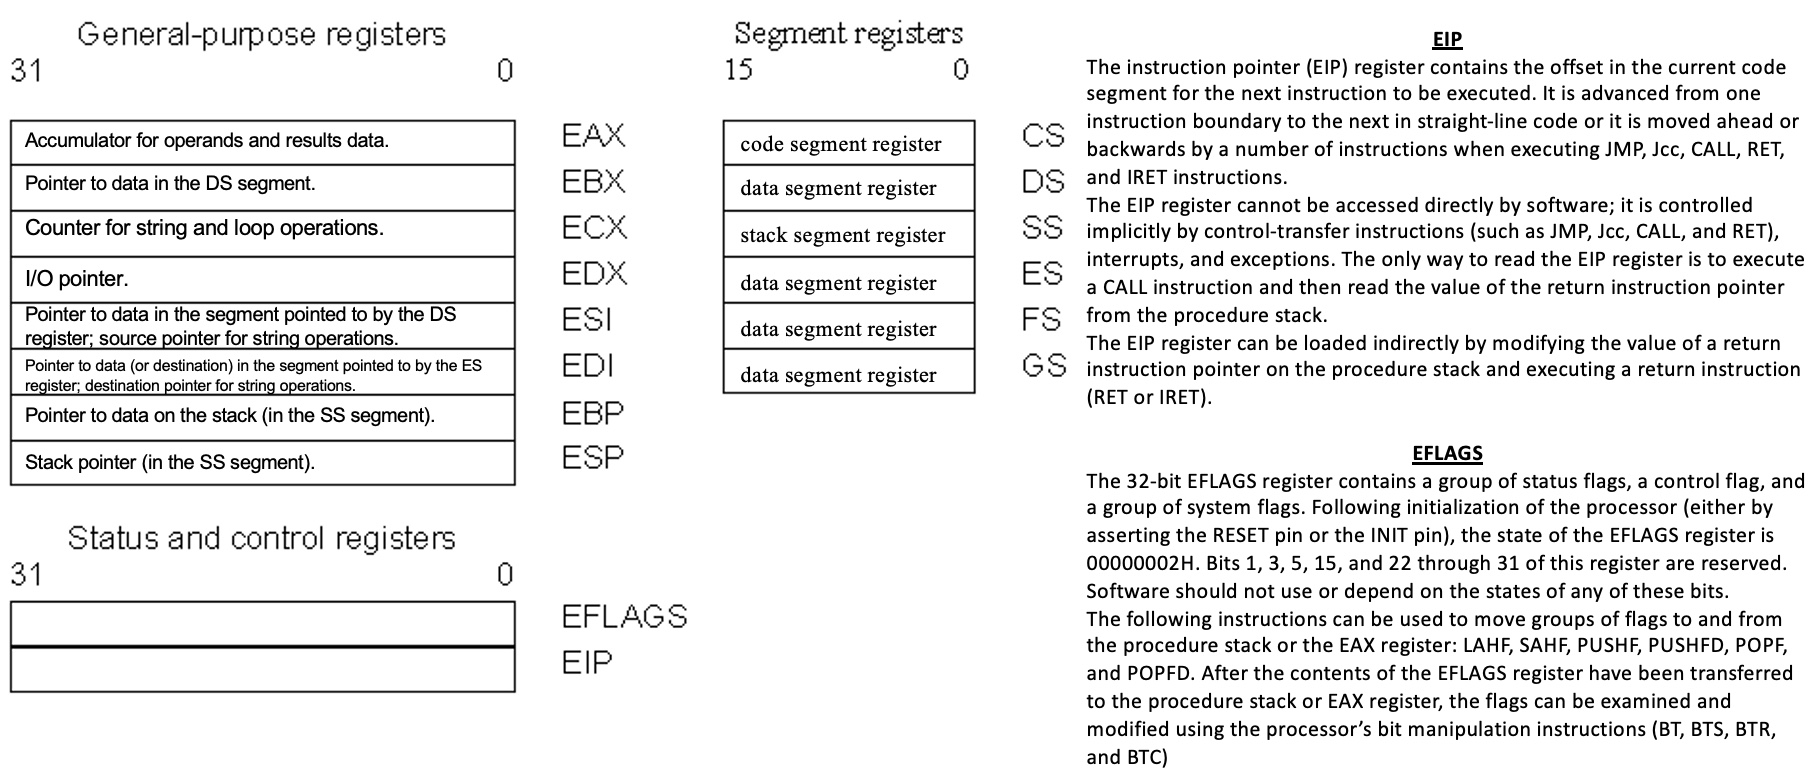
\includegraphics[scale=.27]{Register Diagram.jpeg}
\end{figure}

\subsubsection{The Stack}
The stack is one of two places that a value can be set aside. 
Registers are not managed by a processor and to use one you just need to load a value in it. 
Often there will not be registers available or there is a particular reason a variable will need to reside in RAM instead of in a register. 
That’s when you’d put a variable on the stack instead~\cite{Reversing}.

The stack is a short term storage space in memory that gets utilized by both the CPU and the program. 
It is the spot where short term information gets put when a register can not be used for whatever reason. 
Registers are for the shortest term data while the stack is for the second shortest. 
The stack lives in RAM like all other data and is just a carved out section for intermediate term data. 
Modern operating systems tend to manage multiple stacks at the same time. 
Each of the concurrently running stacks is a representation of a program or thread~\cite{MasteringRE}.

Stacks use Last In First Out data management. 
Items are pushed on the top of the stack and popped from the bottom of the stack. 
Memory in stacks is allocated from the top down where the first in address is allocated and used first while the stack grows backwards towards lower addresses~\cite{Reversing}.

\subsubsection{Flags}
One of the registers you may have noticed from the previous figure is the EFLAGS register. 
This is a collection of special IA-32 registers that contain system and status flags. 
The system flags’ job is to manage the different modes and states of the processor. 
The status flags are what a reverse engineer will typically be more interested in and are used by the processor to record its current logical state~\cite{Reversing}. 
They are often updated by various logical and integer instructions so they can record the outcome of these actions. 
There are also instructions whose operation conditions are dependent on the values for the status flags. 
This is what allows sequences of instructions to run different operations depending on what different input values may be, etc. 

Flags in IA-32 are the crux of conditional code. 
Arithmetic instructions check operand conditions and then set processor flag conditions based on the resulting values. 
There are also sets of instructions designed to read the flags and do different operations based on the value. 
An example of a popular instruction set is Jcc or the Conditional Jump. 
It tests for predefined flag values and then jump depending on whether or not it matches with the specified conditional code~\cite{intelManual}.

\subsubsection{Functions}
Instructions are the actual actions specified in assembly code. 
They are formatted with operation code (opcode) and one or two operands~\cite{Reversing} 
The opcode is what you are asking the computer to do such as MOV or JMP. 
The operand is the parameters that get passed to the opcode or the data being manipulated. 
Certain instructions will have no parameters. Data in assembly comes in three basic forms. 
There are register names, immediate data, and memory addresses. 
Register names are the names of the general purpose registers to be read from or written to like the EAX, EBX, etc. 
Immediate data is constant values that are embedded into the code and usually indicates there was a hard coded value in the source code. 
Memory addresses are the locations of operands stored in RAM. 
It can be hard coded and tell the processor where to read to and write from. 
It could also be a register with a value that will be used as a memory address. 
It is also possible to combine a register with an arithmetic operation and a constant so that there is some base address and then an index offset~\cite{Reversing}.

General purpose instructions are the ones that deal with program flow, logic, arithmetic, string operations, and basic data movement. 
They deal with data stored in memory at the general purpose registers, EFLAGS register, segment registers, and address information stored in memory ~\cite{Reversing}.

The MOV instruction shows up most frequently in most IA-32 instruction sets. 
This one deals with basic data movement. 
It takes in a destination operand and a source operand then moves the data from the source to the destination. 
The sources can be registers, immediate, or memory addresses. 
It is important to note that MOV cannot transfer data through memory, it can only take it out or put it in. 
The destination address can be a memory address (using a register or an immediate) or a register~\cite{Reversing}.




\section{Example Problems}
\subsection{Reversing Hello World}
Before taking on the larger endeavor of reversing a program written in a declarative language (SwiftUI), it’s important to start with the basics. 
Figure [insert figure here] shows a simple ‘Hello World’ program in C. 
To add some complexity, a few random variables and data structures were thrown in as Easter eggs. 
This is the program whose decompilation will be used as a jumping off point.
\begin{figure}[h]
	\caption{Hello World Program}
	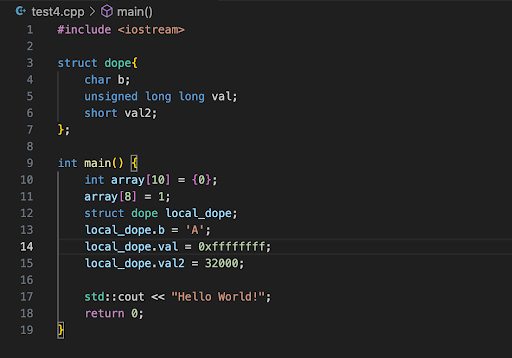
\includegraphics[scale=.75]{HelloWorldSource.png}
\end{figure}
Figure 3 is the decompilation of the program once it was put through Ghidra. 
The first thing to note is how with even a relatively low level language like C, the instructions in the code more than doubled. 
The disassembly being shown in the figure is also only a portion of Ghidra’s output. 
The figure only shows the function section of the program output when imports, exports, labels, classes, etc take up the large majority of the program. 
One important part of reverse engineering is sorting through all of the information to find out what exactly is important to the reverser. 
Some reverse engineers refer to this process as finding the shape and edges of the data. 
\begin{figure}[h]
	\caption{Hello World Disassembly}
	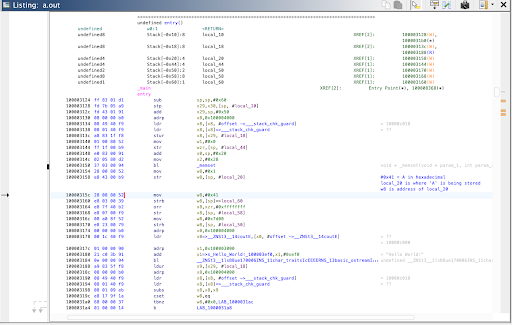
\includegraphics[scale=.3]{HelloWorldGhidra.png}
\end{figure}
With the important section identified, it is time to analyze the assembly code.
One thing to keep in mind with the disassembled code is that all the values will be stored in hexadecimal. 
A good place to start is with the values we know will need to be stored. 
In the array there are 10 variables which all get set to 0, except for the eighth array member which is changed to equal 1. 
In our local\_dope struct there are three variables equal to ‘A’, ‘0xffffffff’, and 32000. 
The highlighted line in the figure shows ‘A’ being stored in the register w8. Shortly after, \#0xfffffff shows up without needing to be translated into hexadecimal. 
\#0x7d000 is the hex for 32000. 
This surface level analysis offers a glimpse into the methodology of more complex reverse engineering. 
Lastly, the 'Hello\_World!' gives us the final piece of information we need to know about what the program is.

\subsection{Crack Me}
The next step in practicing reverse engineering is trying a Crack Me problem. 
Crack Me problems are toy problems designed by other software developers to help reverser's practice their skills. 
Usually there’s an executable that opens up a little puzzle. 
The puzzles usually involve finding a password but can involve any number of things like decryption, key generation, etc. 
This section will cover the process of reverse engineering a simple crack me.

The first step I took in reversing this program was checking the header and libraries as shown in Figure 4 and 5.
\begin{figure}[h]
	\caption{Crack Me Header}
	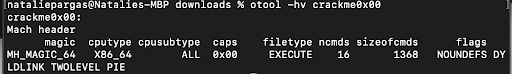
\includegraphics{crackmeheader.png}
\end{figure}
\begin{figure}[h]
	\caption{Crack Me Libraries}
	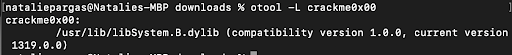
\includegraphics{crackmelibs.png}
\end{figure}

Both of these steps were done with an executable dumping tool called ‘otool’. 
The header information shows that the assembly language being used is x86. 
The library dump shows that the only library being linked is the system library. 
While these tools didn’t offer that much information about this particular program, they are very useful in programs that have more dependencies and more specific assembly languages. 
These dumping tools ended up being vital later in the project because they offered insight into what libraries were being linked from the project's declarative language as well as what assembly language was being used with Apple’s modified version of ARM64. 
Next, otool was used once again to list the strings. 
This is a vital part of reverse engineering and is useful to be able to refer back to during the process. 
Figure 6 shows the result of the string dump.

\begin{figure}[h]
	\caption{Crack Me Strings}
	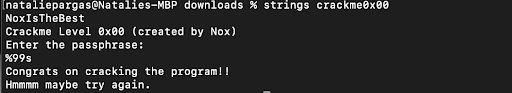
\includegraphics{crackmestrings.png}
\end{figure}

Examining this more closely, you can see that there’s only a few strings that give a very clear idea of what the program is designed to do. 
There’s a random string, the title of the program, a passphrase prompt, a string indicating the expected input, a congratulations message, and an incorrect guess message. 
With just this information, you could easily make an educated guess on what the password is. 
Most likely the passphrase will be the one random string that doesn’t get given easily in the executable. 
But for the sake of gaining understanding of the process, it’s good to go over the decompiled code. 
Figure 7 shows the decompiled code.

\begin{figure}[h]
	\caption{Crack Me Ghidra Disassembly}
	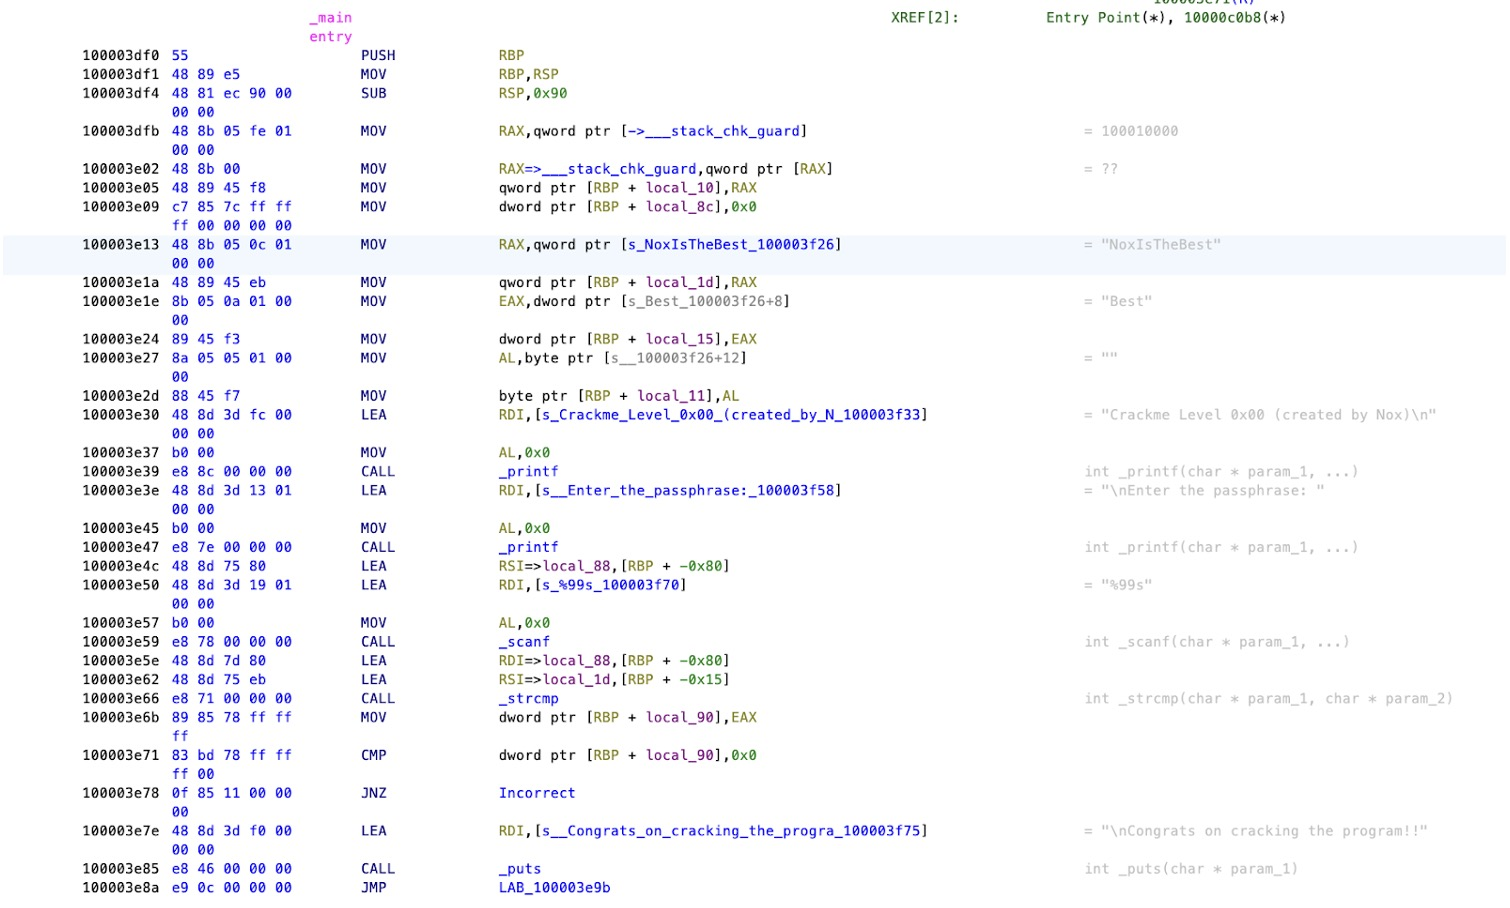
\includegraphics[scale=.3]{crackmeghidra.png}
\end{figure}

The first thing to do is find the entrance into the program. 
Ghidra already labeled the ‘\_main’ at the top but the strings and function calls reaffirm this as the right section to be looking over. 
Next, thinking back to the string dump, it’s likely that the password will be near whatever function takes input. 
Prior knowledge of programming informs the reverser that after getting the user input, the input string will need to be compared to the right answer. 
Thankfully Ghidra was able to identify the function ‘scanf’.

\begin{figure}[h]
	\caption{Crack Me Code Section 1}
	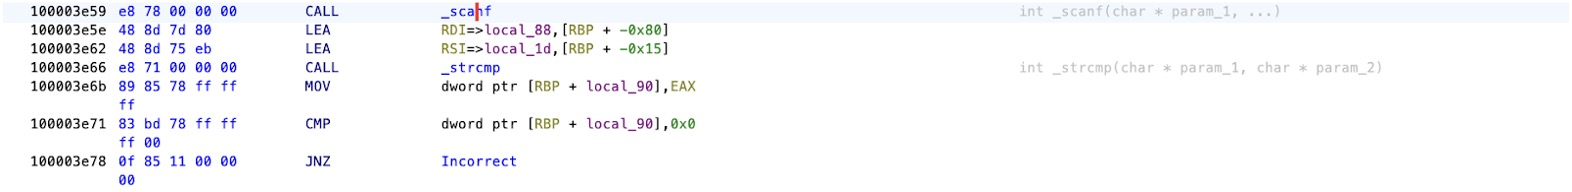
\includegraphics[scale=.3]{crackmescanf.png}
\end{figure}

Inspecting the code section at figure 8, it shows that the variable local\_88 contains the user input. 
This is because it loads a \%99s into the RDI register to prepare for the input directly above where scanf is called. 
RSI has local\_1d loaded into it and that variable is immediately ‘strcmp’ compared to local\_88. Using these clues, one could infer that local\_1d contains the password. 
To verify, a reverser should always retrace and check.

\begin{figure}[h]
	\caption{Crack Me Code Section 2}
	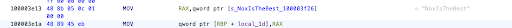
\includegraphics[scale=.3]{crackmeRAX.png}
\end{figure}

The first instance of local\_1d contains the register RAX 9. 
RAX has the qword ptr ‘ s\_NoxIsTheBest\_100003f26’ moved into it right above. 
s\_NoxIsTheBest\_100003f25 only contains the string “NoxIsTheBest”. 
That string is probably the password, but all that’s left is to check. 
Figure 10 shows the result.
\clearpage
\begin{figure}[h!]
	\caption{Crack Me Code Executable}
	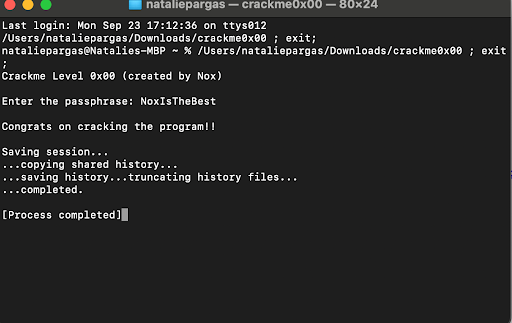
\includegraphics[]{crackmeexe.png}
\end{figure}
The attempt was a success and the crack me was successfully reverse engineered!

\section{Altering the app}
To ensure that I would be able to successfully complete this project, I first needed to confirm that I could alter the app’s behavior in some meaningful way. At the time, the only tools I had available were my MacBook with Android Studio installed. I was running the app on an emulated Android device and quickly found out that in order to use Frida—the dynamic instrumentation toolkit I planned to rely on—I needed to root the emulator. While I had decompiled parts of the app using Jadx, modifying the code that way wasn’t practical. Decompiled code generally can’t be recompiled cleanly, and reconstructing the original logic is both difficult and time-consuming.
Given that Frida was going to be the foundation of my approach for real modifications later on, it made the most sense to start testing with it from the beginning. While it’s true that .xapk files for this app weren’t obfuscated and could have been manually edited and re-signed, that path would have diverged from the strategy I’d ultimately use. Instead, I committed to building out a working Frida workflow right away.

The first step was gathering all necessary tools. This included Frida itself, the frida-server binary compiled for android-arm64 (version 16.7.14), and Objection, a utility built on top of Frida for runtime mobile app exploration. I also installed the Android command line tools directly from Google’s site, which are separate from Android Studio’s full IDE.

With those in place, I turned to setting up a rooted Android emulator. I used rootAVD, a script that modifies emulators to grant root access. Since I was working on an ARM64 Mac, I selected version 12 (Android S) from rootAVD’s compatibility chart. Using Android Studio, I downloaded the system image for API level 28 with an ARM64 architecture. After confirming the image was downloaded, I launched the emulator from the terminal using the emulator command. I first listed the available virtual devices, then ran the appropriate command to launch the desired AVD.

Inside the rootAVD directory, I ran the script by typing ./rootAVD.sh. I listed all the AVDs and selected the correct ramdisk.img from the path system-images/android-28/default/arm64-v8a. If everything was patched successfully, the emulator would shut down and then boot up again normally. A grey or black screen during boot was a sign that something had gone wrong. Once the emulator was running again, I verified root access using ADB. I ran adb shell, then typed su, followed by whoami. If the output returned "root," that meant the emulator was successfully rooted.

At that point, I was ready to run Objection. I launched it in a new terminal window by attaching it to the app’s process using the command objection -g com.loreal.ysl.perso.lips explore. If everything was working correctly, Objection would connect to the app, allowing for runtime exploration and testing.

Next, I needed to get frida-server running on the device. I navigated to the folder where the binary was located and made it executable with chmod +x. Then I pushed it to the emulator’s file system using ADB. Specifically, I placed it in /data/local/tmp using the command adb push frida-server-16.7.14-android-arm64 /data/local/tmp/frida-server. After entering the device shell and switching to root again with su, I launched the server in the background using \texttt{./frida-server \&}. A successful start would return a process ID.

With the Frida server running and everything hooked up, I tested a simple proof-of-concept string replacement. I began by choosing the string I wanted to replace: “No activities yet.” To work with it at the memory level, I converted the string to hexadecimal using echo -n "No activities yet" | xxd -p, which gave me the raw hex representation of the text. I then used Frida’s memory search capabilities to locate that hex sequence in the app’s memory.

Next, I decided on the replacement string—“Natalie activities”—and repeated the process to convert it to hex using the same xxd command. Then I retrieved the process ID (PID) of the running app using adb shell pidof com.loreal.ysl.perso.lips. With that PID, I ran the Frida script I had written to replace the original string with the new one. The command was \texttt{frida -U -p <PID> -l replace\_textview.js}. Occasionally, Frida throws unhelpful syntax errors—like missing semicolons—that don’t actually affect runtime behavior. Even if such an error appeared, I would go back to the app, let it load, and check if the text had been replaced. And in this case, once the relevant screen rendered, the string had indeed been swapped out, confirming that the setup was working.

% TODO: \usepackage{graphicx} required
\begin{figure}
	\centering
	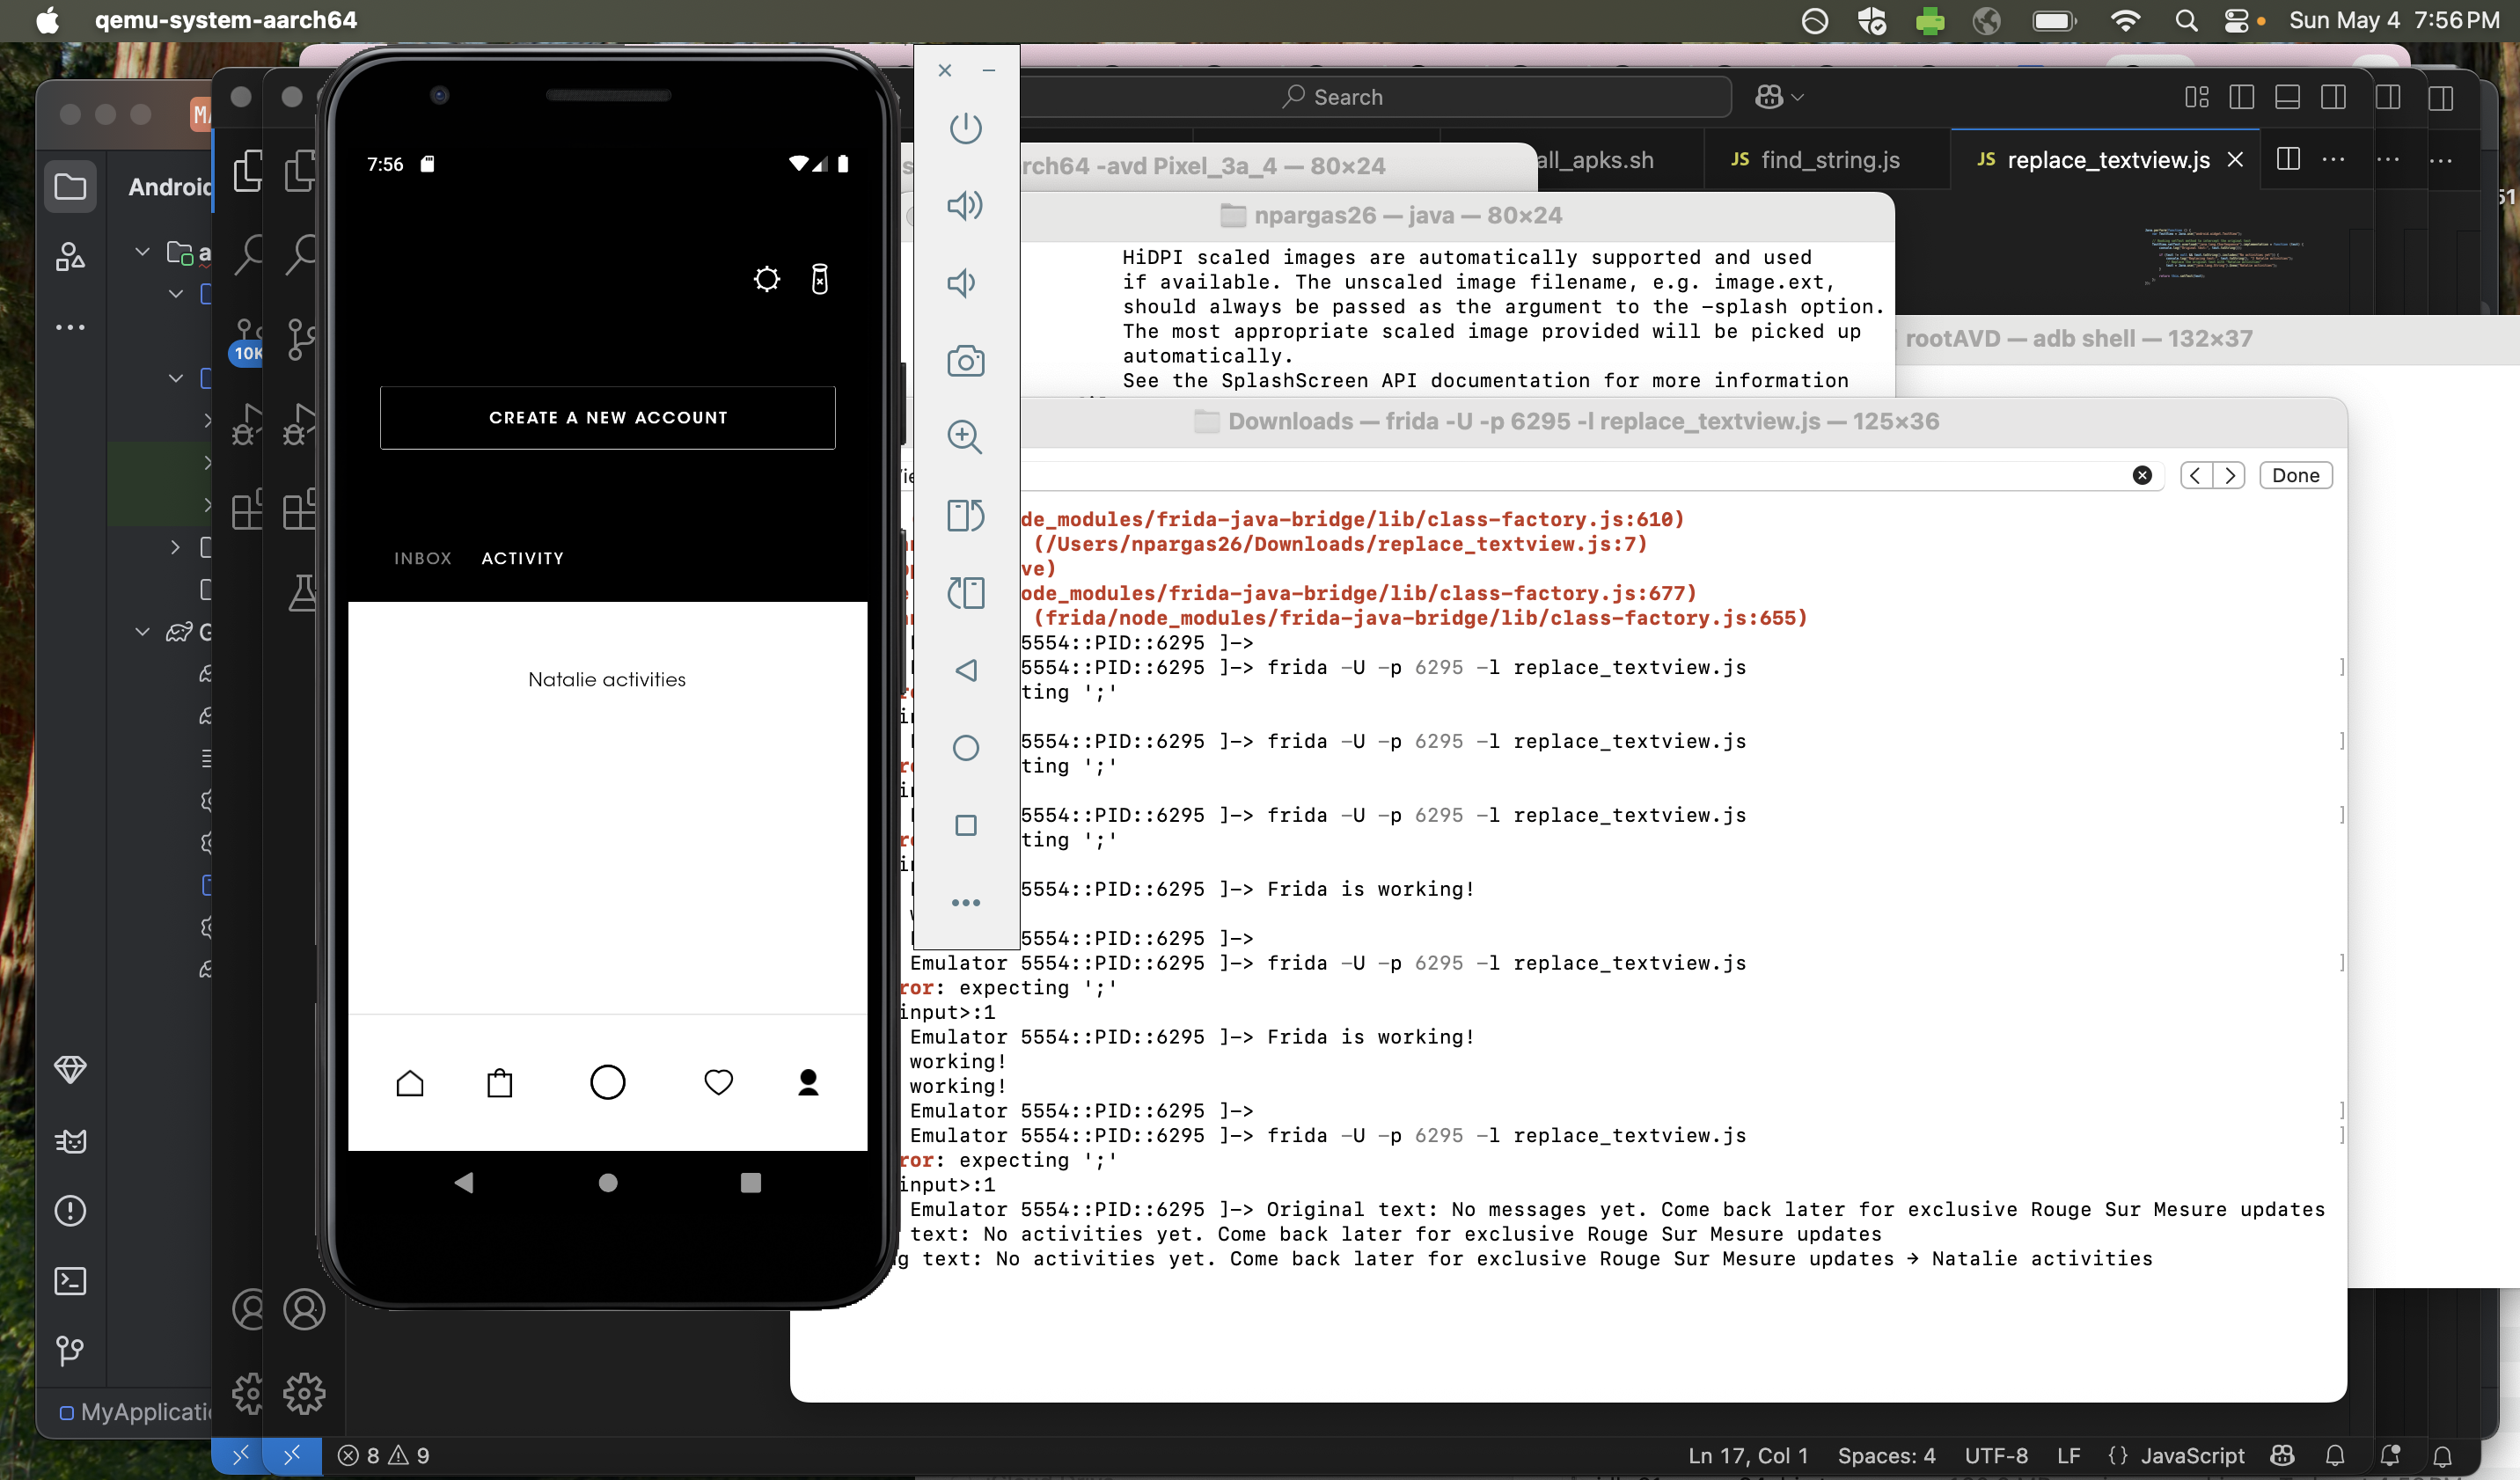
\includegraphics[scale=.17]{Natalie_activities}
	\caption{}
	\label{fig:natalieactivities}
\end{figure}
